\paragraph{Measured results.}
Table~\ref{tab:matched-primary} reports the predeclared 20\% target. A dash means an unresolved reference or no eligible tested budget; it never denotes an infinite speedup. The analytic-source and incremental-grid extensions were introduced after the first housing result and frozen before their own measurements. Their results are therefore separate diagnostic extensions, not retroactively part of the initial protocol.
\begin{table}[t]\centering\small
\caption{Calibration results at the 20\% reference-relative accuracy target. Times include every batch through the listed query count. MG is the fastest eligible tested resolution and reuse variant. RB denotes exact-source integration in ideal arithmetic. All quantities are empirical; source restrictions and numerical-reference gates apply.}
\label{tab:matched-primary}
\begin{tabular}{llrrrrrr}\toprule
Object & State & Queries & TWoS (s) & TWoS--RB (s) & MG (s) & MG/RB & RB paths\\\midrule
Branch & edited & 8 & 0.997 & 0.823 & 0.049 & 0.06 & 4096\\
Branch & edited & 512 & 53.502 & 13.063 & 0.053 & 0.00 & 1024\\
Branch & original & 8 & 0.982 & 0.877 & 0.090 & 0.10 & 4096\\
Branch & original & 512 & 49.404 & 11.476 & 0.095 & 0.01 & 1024\\
Bunny & edited & 8 & 1.635 & 0.409 & 0.122 & 0.30 & 1024\\
Bunny & edited & 512 & 77.790 & 17.474 & 0.128 & 0.01 & 1024\\
Bunny & original & 8 & 1.406 & 0.322 & 0.201 & 0.62 & 1024\\
Bunny & original & 512 & 71.133 & 18.535 & 0.208 & 0.01 & 1024\\
Bunny compliance & edited & 8 & -- & 0.023 & 0.073 & 3.17 & 64\\
Bunny compliance & edited & 512 & -- & 4.372 & 0.079 & 0.02 & 256\\
Bunny compliance & original & 8 & -- & 0.028 & 0.116 & 4.19 & 64\\
Bunny compliance & original & 512 & -- & 4.430 & 0.120 & 0.03 & 256\\
Housing & edited & 8 & -- & 0.084 & 0.031 & 0.37 & 1024\\
Housing & edited & 512 & 22.283 & 4.875 & 0.036 & 0.01 & 1024\\
Housing & original & 8 & -- & 0.084 & 0.085 & 1.02 & 1024\\
Housing & original & 512 & 21.718 & 4.595 & 0.089 & 0.02 & 1024\\
Ring & edited & 8 & -- & 0.255 & 0.039 & 0.15 & 1024\\
Ring & edited & 512 & 54.190 & 11.832 & 0.043 & 0.00 & 1024\\
Ring & original & 8 & -- & 0.239 & 0.102 & 0.43 & 1024\\
Ring & original & 512 & 49.844 & 12.061 & 0.109 & 0.01 & 1024\\
\bottomrule\end{tabular}\end{table}
\begin{table}[t]\centering\small
\caption{Independent reference diagnostics. Refinement discrepancies are shown at 8 and 512 sites; the 32-site Monte Carlo diagnostic is common to each state. Values are percentages. These quantities are not rigorous error bounds.}
\begin{tabular}{llrrrr}\toprule Object & State & $\delta_8$ & $\delta_{512}$ & MC SE norm & MC--grid discrepancy\\\midrule
Branch & edited & 1.34 & 1.29 & 3.07 & 5.37\\
Branch & original & 1.34 & 1.29 & 3.35 & 5.62\\
Bunny & edited & 0.84 & 0.74 & 3.79 & 2.45\\
Bunny & original & 0.84 & 0.74 & 3.86 & 2.64\\
Bunny compliance & edited & 1.16 & 1.27 & 0.57 & 2.49\\
Bunny compliance & original & 1.16 & 1.27 & 0.56 & 2.44\\
Housing & edited & 0.70 & 3.03 & 2.87 & 6.11\\
Housing & original & 0.70 & 3.03 & 2.87 & 6.11\\
Ring & edited & 1.36 & 1.03 & 2.98 & 7.01\\
Ring & original & 1.36 & 1.03 & 2.98 & 7.01\\
\bottomrule\end{tabular}\end{table}
\begin{figure}[p]\centering
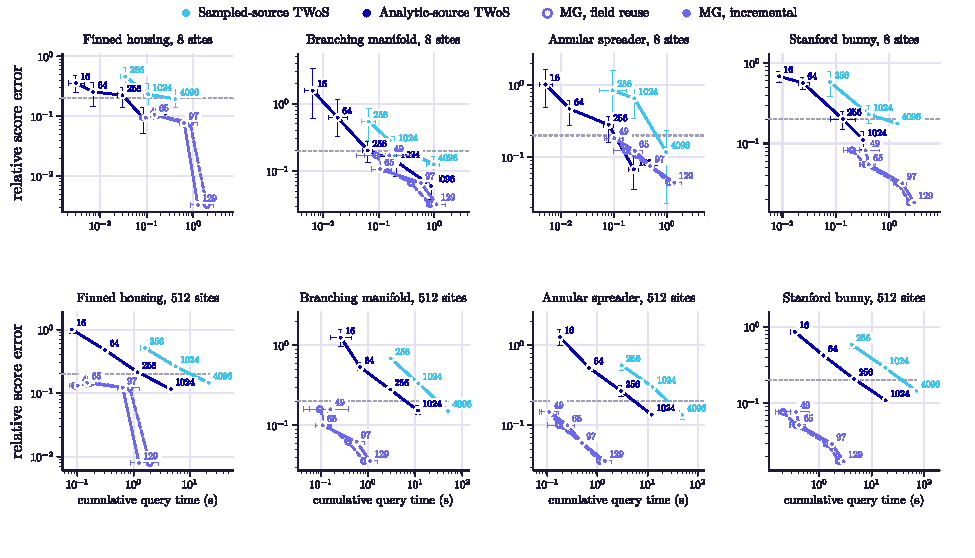
\includegraphics[width=\textwidth]{figures/matched-accuracy-original.pdf}
\caption{All measured budgets on the original domain, at 8 sites (top) and 512 sites (bottom). Bars are pointwise 95\% bootstrap intervals over five seeds; they exclude numerical-reference bias. Dashed horizontal lines mark the 20\% target before applying the independent reference gates. Numbers label path counts or longest-axis grid counts. Original and source-integrated TWoS and both grid reuse variants are retained.}\end{figure}
\begin{figure}[p]\centering
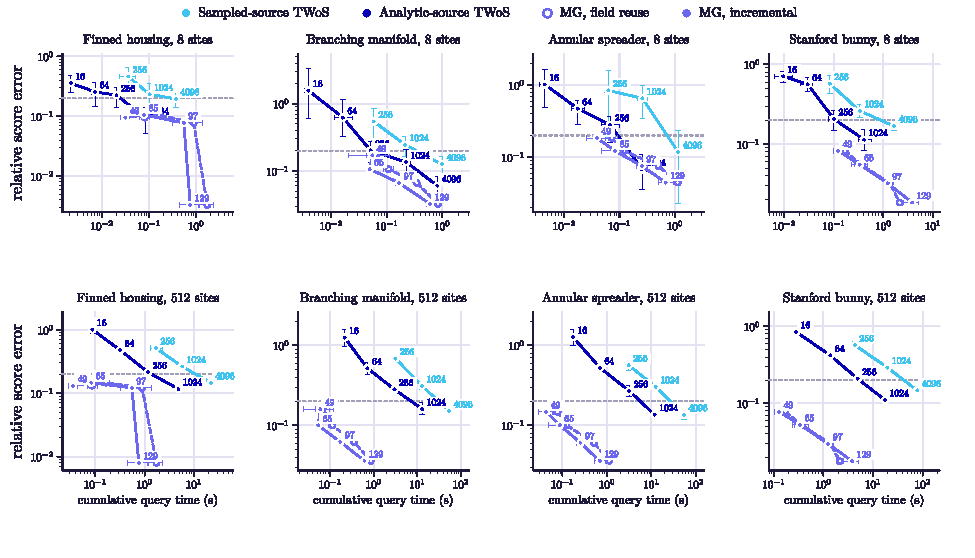
\includegraphics[width=\textwidth]{figures/matched-accuracy-edited.pdf}
\caption{All measured budgets on the edited domain, at 8 sites (top) and 512 sites (bottom). Bars are pointwise 95\% bootstrap intervals over five seeds; they exclude numerical-reference bias. Dashed horizontal lines mark the 20\% target before applying the independent reference gates. Numbers label path counts or longest-axis grid counts. Original and source-integrated TWoS and both grid reuse variants are retained.}\end{figure}
\begin{figure}[p]\centering
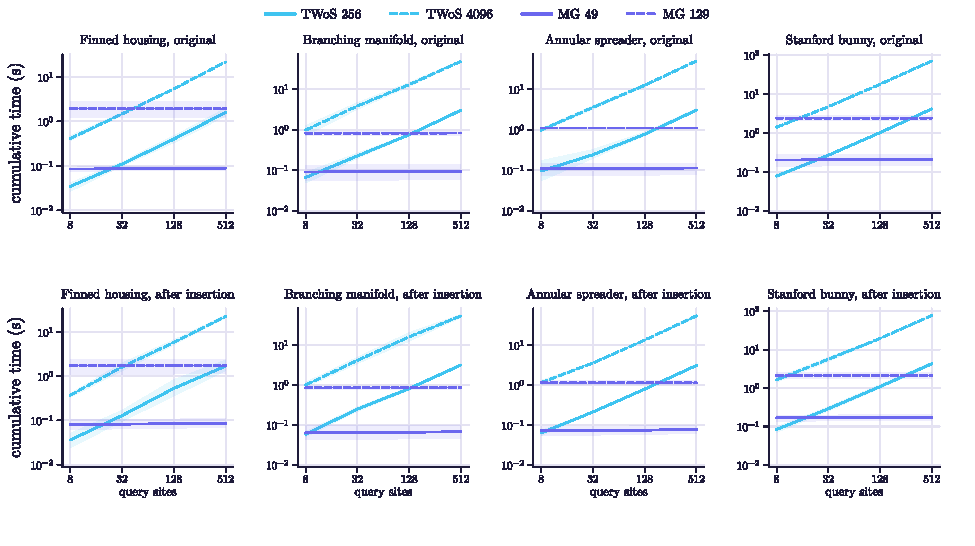
\includegraphics[width=\textwidth]{figures/matched-accuracy-scaling.pdf}
\caption{Measured query-count scaling at fixed budgets in the initially frozen sweep. Shaded bands show pointwise 95\% bootstrap intervals for mean time. Original-source TWoS scales with the number of sites, whereas solved-field multigrid amortizes its setup. These fixed-budget curves do not assert matched accuracy.}\end{figure}
\paragraph{Fresh-seed confirmation and its failures.}
The four apparent 20\%-target wins selected from calibration did not pass both fresh-seed rules. The three compliance cases exceeded the mean-error upper-endpoint threshold; the housing timing interval included no advantage. We then declared a separate, fixed 256-path follow-up for both eight-site compliance states, with 20 further fresh seeds and no subsequent budget search. All results are retained below. These pointwise bootstrap checks are not simultaneous confidence guarantees.
\begin{table}[t]\centering\small
\caption{Fresh-seed query confirmations. Times exclude common geometry loading. Error upper endpoints and speed intervals use 10,000 paired bootstrap resamples of 20 seeds. Passing requires error upper endpoint $\leq20\%$ and speed-ratio lower endpoint $>1$. Every row uses MG49.}
\setlength{\tabcolsep}{3.2pt}
\begin{tabular}{llrrrrrr}\toprule Workload / state & Stage & Sites & Paths & TWoS / MG (ms) & Error upper & MG/TWoS interval & Pass\\\midrule
Bunny compliance / edited & Selected & 8 & 64 & 23.3 / 78.4 & 21.8\% & [2.51, 4.57] & no\\
Bunny compliance / original & Selected & 8 & 64 & 28.7 / 341.3 & 21.3\% & [6.21, 19.36] & no\\
Bunny compliance / original & Selected & 32 & 64 & 74.0 / 136.8 & 20.8\% & [1.58, 2.13] & no\\
Housing / original & Selected & 8 & 1024 & 137.4 / 131.9 & 13.6\% & [0.58, 1.54] & no\\
Bunny compliance / edited & Fixed 256 & 8 & 256 & 83.1 / 72.8 & 10.3\% & [0.69, 1.11] & no\\
Bunny compliance / original & Fixed 256 & 8 & 256 & 89.9 / 113.9 & 10.2\% & [1.05, 1.50] & yes\\
\bottomrule\end{tabular}\end{table}
